% Options for packages loaded elsewhere
\PassOptionsToPackage{unicode}{hyperref}
\PassOptionsToPackage{hyphens}{url}
%
\documentclass[
]{article}
\usepackage{amsmath,amssymb}
\usepackage{iftex}
\ifPDFTeX
  \usepackage[T1]{fontenc}
  \usepackage[utf8]{inputenc}
  \usepackage{textcomp} % provide euro and other symbols
\else % if luatex or xetex
  \usepackage{unicode-math} % this also loads fontspec
  \defaultfontfeatures{Scale=MatchLowercase}
  \defaultfontfeatures[\rmfamily]{Ligatures=TeX,Scale=1}
\fi
\usepackage{lmodern}
\ifPDFTeX\else
  % xetex/luatex font selection
\fi
% Use upquote if available, for straight quotes in verbatim environments
\IfFileExists{upquote.sty}{\usepackage{upquote}}{}
\IfFileExists{microtype.sty}{% use microtype if available
  \usepackage[]{microtype}
  \UseMicrotypeSet[protrusion]{basicmath} % disable protrusion for tt fonts
}{}
\makeatletter
\@ifundefined{KOMAClassName}{% if non-KOMA class
  \IfFileExists{parskip.sty}{%
    \usepackage{parskip}
  }{% else
    \setlength{\parindent}{0pt}
    \setlength{\parskip}{6pt plus 2pt minus 1pt}}
}{% if KOMA class
  \KOMAoptions{parskip=half}}
\makeatother
\usepackage{xcolor}
\usepackage[margin=1in]{geometry}
\usepackage{color}
\usepackage{fancyvrb}
\newcommand{\VerbBar}{|}
\newcommand{\VERB}{\Verb[commandchars=\\\{\}]}
\DefineVerbatimEnvironment{Highlighting}{Verbatim}{commandchars=\\\{\}}
% Add ',fontsize=\small' for more characters per line
\usepackage{framed}
\definecolor{shadecolor}{RGB}{248,248,248}
\newenvironment{Shaded}{\begin{snugshade}}{\end{snugshade}}
\newcommand{\AlertTok}[1]{\textcolor[rgb]{0.94,0.16,0.16}{#1}}
\newcommand{\AnnotationTok}[1]{\textcolor[rgb]{0.56,0.35,0.01}{\textbf{\textit{#1}}}}
\newcommand{\AttributeTok}[1]{\textcolor[rgb]{0.13,0.29,0.53}{#1}}
\newcommand{\BaseNTok}[1]{\textcolor[rgb]{0.00,0.00,0.81}{#1}}
\newcommand{\BuiltInTok}[1]{#1}
\newcommand{\CharTok}[1]{\textcolor[rgb]{0.31,0.60,0.02}{#1}}
\newcommand{\CommentTok}[1]{\textcolor[rgb]{0.56,0.35,0.01}{\textit{#1}}}
\newcommand{\CommentVarTok}[1]{\textcolor[rgb]{0.56,0.35,0.01}{\textbf{\textit{#1}}}}
\newcommand{\ConstantTok}[1]{\textcolor[rgb]{0.56,0.35,0.01}{#1}}
\newcommand{\ControlFlowTok}[1]{\textcolor[rgb]{0.13,0.29,0.53}{\textbf{#1}}}
\newcommand{\DataTypeTok}[1]{\textcolor[rgb]{0.13,0.29,0.53}{#1}}
\newcommand{\DecValTok}[1]{\textcolor[rgb]{0.00,0.00,0.81}{#1}}
\newcommand{\DocumentationTok}[1]{\textcolor[rgb]{0.56,0.35,0.01}{\textbf{\textit{#1}}}}
\newcommand{\ErrorTok}[1]{\textcolor[rgb]{0.64,0.00,0.00}{\textbf{#1}}}
\newcommand{\ExtensionTok}[1]{#1}
\newcommand{\FloatTok}[1]{\textcolor[rgb]{0.00,0.00,0.81}{#1}}
\newcommand{\FunctionTok}[1]{\textcolor[rgb]{0.13,0.29,0.53}{\textbf{#1}}}
\newcommand{\ImportTok}[1]{#1}
\newcommand{\InformationTok}[1]{\textcolor[rgb]{0.56,0.35,0.01}{\textbf{\textit{#1}}}}
\newcommand{\KeywordTok}[1]{\textcolor[rgb]{0.13,0.29,0.53}{\textbf{#1}}}
\newcommand{\NormalTok}[1]{#1}
\newcommand{\OperatorTok}[1]{\textcolor[rgb]{0.81,0.36,0.00}{\textbf{#1}}}
\newcommand{\OtherTok}[1]{\textcolor[rgb]{0.56,0.35,0.01}{#1}}
\newcommand{\PreprocessorTok}[1]{\textcolor[rgb]{0.56,0.35,0.01}{\textit{#1}}}
\newcommand{\RegionMarkerTok}[1]{#1}
\newcommand{\SpecialCharTok}[1]{\textcolor[rgb]{0.81,0.36,0.00}{\textbf{#1}}}
\newcommand{\SpecialStringTok}[1]{\textcolor[rgb]{0.31,0.60,0.02}{#1}}
\newcommand{\StringTok}[1]{\textcolor[rgb]{0.31,0.60,0.02}{#1}}
\newcommand{\VariableTok}[1]{\textcolor[rgb]{0.00,0.00,0.00}{#1}}
\newcommand{\VerbatimStringTok}[1]{\textcolor[rgb]{0.31,0.60,0.02}{#1}}
\newcommand{\WarningTok}[1]{\textcolor[rgb]{0.56,0.35,0.01}{\textbf{\textit{#1}}}}
\usepackage{graphicx}
\makeatletter
\def\maxwidth{\ifdim\Gin@nat@width>\linewidth\linewidth\else\Gin@nat@width\fi}
\def\maxheight{\ifdim\Gin@nat@height>\textheight\textheight\else\Gin@nat@height\fi}
\makeatother
% Scale images if necessary, so that they will not overflow the page
% margins by default, and it is still possible to overwrite the defaults
% using explicit options in \includegraphics[width, height, ...]{}
\setkeys{Gin}{width=\maxwidth,height=\maxheight,keepaspectratio}
% Set default figure placement to htbp
\makeatletter
\def\fps@figure{htbp}
\makeatother
\setlength{\emergencystretch}{3em} % prevent overfull lines
\providecommand{\tightlist}{%
  \setlength{\itemsep}{0pt}\setlength{\parskip}{0pt}}
\setcounter{secnumdepth}{-\maxdimen} % remove section numbering
\ifLuaTeX
  \usepackage{selnolig}  % disable illegal ligatures
\fi
\IfFileExists{bookmark.sty}{\usepackage{bookmark}}{\usepackage{hyperref}}
\IfFileExists{xurl.sty}{\usepackage{xurl}}{} % add URL line breaks if available
\urlstyle{same}
\hypersetup{
  pdftitle={Case Study 3: Geographic distribution of crime in Mexico},
  pdfauthor={David Buil-Gil and Reka Solymosi},
  hidelinks,
  pdfcreator={LaTeX via pandoc}}

\title{Case Study 3: Geographic distribution of crime in Mexico}
\author{David Buil-Gil and Reka Solymosi}
\date{2024-01-25}

\begin{document}
\maketitle

CONTEXT

We analyse police-recorded crime data made available in the webside of
the Mexican Government
(\url{https://www.gob.mx/sesnsp/acciones-y-programas/datos-abiertos-de-incidencia-delictiva?state=published}).

We begin by loading the required packages in R:

\begin{Shaded}
\begin{Highlighting}[]
\FunctionTok{library}\NormalTok{(here)}
\FunctionTok{library}\NormalTok{(dplyr)}
\FunctionTok{library}\NormalTok{(ggplot2)}
\end{Highlighting}
\end{Shaded}

We open this dataset and select only those rows that refer to our crime
type of interest: kidnappings (or `secuestro' in Spanish). We are
particularly interested in exploring the geographic distribution of
crimes in 2017; the last year when data was made available.

\begin{Shaded}
\begin{Highlighting}[]
\CommentTok{\#Read csv file with crime data}
\NormalTok{data\_Mexico }\OtherTok{\textless{}{-}} \FunctionTok{read.csv}\NormalTok{(}\FunctionTok{here}\NormalTok{(}\StringTok{"data/IDM\_nov2023.csv"}\NormalTok{))}

\CommentTok{\#Select crime type of interest in dataset, and only records for 2017}
\NormalTok{data\_Mexico }\OtherTok{\textless{}{-}}\NormalTok{ data\_Mexico }\SpecialCharTok{\%\textgreater{}\%}
  \FunctionTok{filter}\NormalTok{(MODALIDAD }\SpecialCharTok{==} \StringTok{"PRIV. DE LA LIBERTAD (SECUESTRO)"}\NormalTok{) }\SpecialCharTok{\%\textgreater{}\%}
  \FunctionTok{filter}\NormalTok{(ANO }\SpecialCharTok{==} \DecValTok{2017}\NormalTok{)}
\end{Highlighting}
\end{Shaded}

Calculate number of crimes each year in each state (`ENTIDAD' in the
database).

\begin{Shaded}
\begin{Highlighting}[]
\CommentTok{\#Calculate number of crimes across months}
\NormalTok{data\_Mexico }\OtherTok{\textless{}{-}}\NormalTok{ data\_Mexico }\SpecialCharTok{\%\textgreater{}\%}
  \FunctionTok{mutate}\NormalTok{(}\AttributeTok{freq =} \FunctionTok{rowSums}\NormalTok{(}\FunctionTok{select}\NormalTok{(., }\DecValTok{8}\SpecialCharTok{:}\DecValTok{19}\NormalTok{), }\AttributeTok{na.rm =} \ConstantTok{TRUE}\NormalTok{))}

\CommentTok{\#Select variables of interest only}
\NormalTok{data\_Mexico }\OtherTok{\textless{}{-}}\NormalTok{ data\_Mexico }\SpecialCharTok{\%\textgreater{}\%}
  \FunctionTok{select}\NormalTok{(ANO, ENTIDAD, TIPO, freq)}

\CommentTok{\#Calculate number of crimes in each state}
\NormalTok{data\_Mexico\_states }\OtherTok{\textless{}{-}}\NormalTok{ data\_Mexico }\SpecialCharTok{\%\textgreater{}\%}
  \FunctionTok{group\_by}\NormalTok{(ENTIDAD) }\SpecialCharTok{\%\textgreater{}\%}
  \FunctionTok{summarize}\NormalTok{(}\AttributeTok{freq =} \FunctionTok{sum}\NormalTok{(freq))}
\end{Highlighting}
\end{Shaded}

We have now created a new database called `data\_Mexico\_states' which
includes the count of kidnappings for each state in 2017. We can execute
`top\_n(data\_Mexico\_states, 3, freq)' and observe that the State of
Mexico concentrates the largest number of kidnappings, 173, followed by
Veracruz, with 172. On the other end, Yucatan recorded 0 kidnappings in
2017. On average, 35.9 kidnappings were recorded across the 32 states of
Mexico (`mean(data\_Mexico\_states\$freq').

This however may mark \ldots{} need for rates. We calculate rates of
kidnappings per 100,000 residents.

Population:
\url{https://www.inegi.org.mx/app/tabulados/default.html?nc=mdemo02}

\begin{Shaded}
\begin{Highlighting}[]
\CommentTok{\#Read csv file with population data}
\NormalTok{population }\OtherTok{\textless{}{-}} \FunctionTok{read.csv}\NormalTok{(}\FunctionTok{here}\NormalTok{(}\StringTok{"data/Population2010.csv"}\NormalTok{))}

\CommentTok{\#Merge with crime data and calculate crime rates}
\NormalTok{data\_Mexico\_states }\OtherTok{\textless{}{-}}\NormalTok{ data\_Mexico\_states }\SpecialCharTok{\%\textgreater{}\%}
  \FunctionTok{left\_join}\NormalTok{(population, }\AttributeTok{by =} \FunctionTok{c}\NormalTok{(}\StringTok{"ENTIDAD"} \OtherTok{=} \StringTok{"STATE"}\NormalTok{)) }\SpecialCharTok{\%\textgreater{}\%}
  \FunctionTok{mutate}\NormalTok{(}\AttributeTok{crime\_rate =}\NormalTok{ freq }\SpecialCharTok{/}\NormalTok{ Population2010 }\SpecialCharTok{*} \DecValTok{100000}\NormalTok{)}
\end{Highlighting}
\end{Shaded}

According to calculated crime rates, the states with the highest rates
of kidnappings per capita are Zacatecas and Tamaulipas, both with over 4
kidnappings per 100,000 residents.

Finally, we want to display crime rates in maps.

Source: \url{https://github.com/strotgen/mexico-leaflet/}

\begin{Shaded}
\begin{Highlighting}[]
\FunctionTok{library}\NormalTok{(sf)}
\end{Highlighting}
\end{Shaded}

\begin{verbatim}
## Linking to GEOS 3.11.2, GDAL 3.6.2, PROJ 9.2.0; sf_use_s2() is TRUE
\end{verbatim}

\begin{Shaded}
\begin{Highlighting}[]
\CommentTok{\#Read geojson of Mexico states}
\CommentTok{\#states\_geojson \textless{}{-} st\_read("https://github.com/strotgen/mexico{-}leaflet/blob/master/states.geojson")}
\NormalTok{states\_geojson }\OtherTok{\textless{}{-}} \FunctionTok{st\_read}\NormalTok{(}\FunctionTok{here}\NormalTok{(}\StringTok{"data/states.geojson"}\NormalTok{))}
\end{Highlighting}
\end{Shaded}

\begin{verbatim}
## Reading layer `states' from data source 
##   `\\nask.man.ac.uk\home$\Documents\GitHub\crim-data-south2\data\states.geojson' 
##   using driver `GeoJSON'
## Simple feature collection with 32 features and 3 fields
## Geometry type: MULTIPOLYGON
## Dimension:     XY
## Bounding box:  xmin: -118.4 ymin: 14.5321 xmax: -86.72404 ymax: 32.71865
## Geodetic CRS:  WGS 84
\end{verbatim}

\begin{Shaded}
\begin{Highlighting}[]
\CommentTok{\#Merge crime rates with geojson file}
\NormalTok{states\_geojson }\OtherTok{\textless{}{-}}\NormalTok{ states\_geojson }\SpecialCharTok{\%\textgreater{}\%}
  \FunctionTok{mutate}\NormalTok{(}\AttributeTok{state\_name =} \FunctionTok{toupper}\NormalTok{(state\_name), }\CommentTok{\#capital letters for consistency}
         \AttributeTok{state\_name =} \FunctionTok{recode}\NormalTok{(state\_name, }\CommentTok{\#rename some states for consistency}
                             \StringTok{\textquotesingle{}DISTRITO FEDERAL\textquotesingle{}} \OtherTok{=} \StringTok{\textquotesingle{}CIUDAD DE MEXICO\textquotesingle{}}\NormalTok{,}
                             \StringTok{\textquotesingle{}MÉXICO\textquotesingle{}} \OtherTok{=} \StringTok{\textquotesingle{}MEXICO\textquotesingle{}}\NormalTok{,}
                             \StringTok{\textquotesingle{}MICHOACÁN DE OCAMPO\textquotesingle{}} \OtherTok{=} \StringTok{\textquotesingle{}MICHOACAN\textquotesingle{}}\NormalTok{,}
                             \StringTok{\textquotesingle{}QUERÉTARO\textquotesingle{}} \OtherTok{=} \StringTok{\textquotesingle{}QUERETARO\textquotesingle{}}\NormalTok{,}
                             \StringTok{\textquotesingle{}SAN LUIS POTOSÍ\textquotesingle{}} \OtherTok{=} \StringTok{\textquotesingle{}SAN LUIS POTOSI\textquotesingle{}}\NormalTok{,}
                             \StringTok{\textquotesingle{}VERACRUZ DE IGNACIO DE LA LLAVE\textquotesingle{}} \OtherTok{=} \StringTok{\textquotesingle{}VERACRUZ\textquotesingle{}}\NormalTok{,}
                             \StringTok{\textquotesingle{}NUEVO LEÓN\textquotesingle{}} \OtherTok{=} \StringTok{\textquotesingle{}NUEVO LEON\textquotesingle{}}\NormalTok{,}
                             \StringTok{\textquotesingle{}COAHUILA DE ZARAGOZA\textquotesingle{}} \OtherTok{=} \StringTok{\textquotesingle{}COAHUILA\textquotesingle{}}\NormalTok{,}
                             \StringTok{\textquotesingle{}YUCATÁN\textquotesingle{}} \OtherTok{=} \StringTok{\textquotesingle{}YUCATAN\textquotesingle{}}\NormalTok{)) }\SpecialCharTok{\%\textgreater{}\%} 
  \FunctionTok{left\_join}\NormalTok{(data\_Mexico\_states, }\AttributeTok{by =} \FunctionTok{c}\NormalTok{(}\StringTok{"state\_name"} \OtherTok{=} \StringTok{"ENTIDAD"}\NormalTok{))}
\end{Highlighting}
\end{Shaded}

\begin{Shaded}
\begin{Highlighting}[]
\FunctionTok{ggplot}\NormalTok{(}\AttributeTok{data =}\NormalTok{ states\_geojson) }\SpecialCharTok{+}
  \FunctionTok{ggtitle}\NormalTok{(}\StringTok{"Rate of kidnappings per 100,000 residents in Mexico states"}\NormalTok{) }\SpecialCharTok{+}
  \FunctionTok{geom\_sf}\NormalTok{(}\FunctionTok{aes}\NormalTok{(}\AttributeTok{fill =}\NormalTok{ crime\_rate)) }\SpecialCharTok{+}
  \FunctionTok{scale\_fill\_viridis}\NormalTok{(}\AttributeTok{option =} \StringTok{"magma"}\NormalTok{)}\SpecialCharTok{+}
  \FunctionTok{theme\_void}\NormalTok{()}
\end{Highlighting}
\end{Shaded}

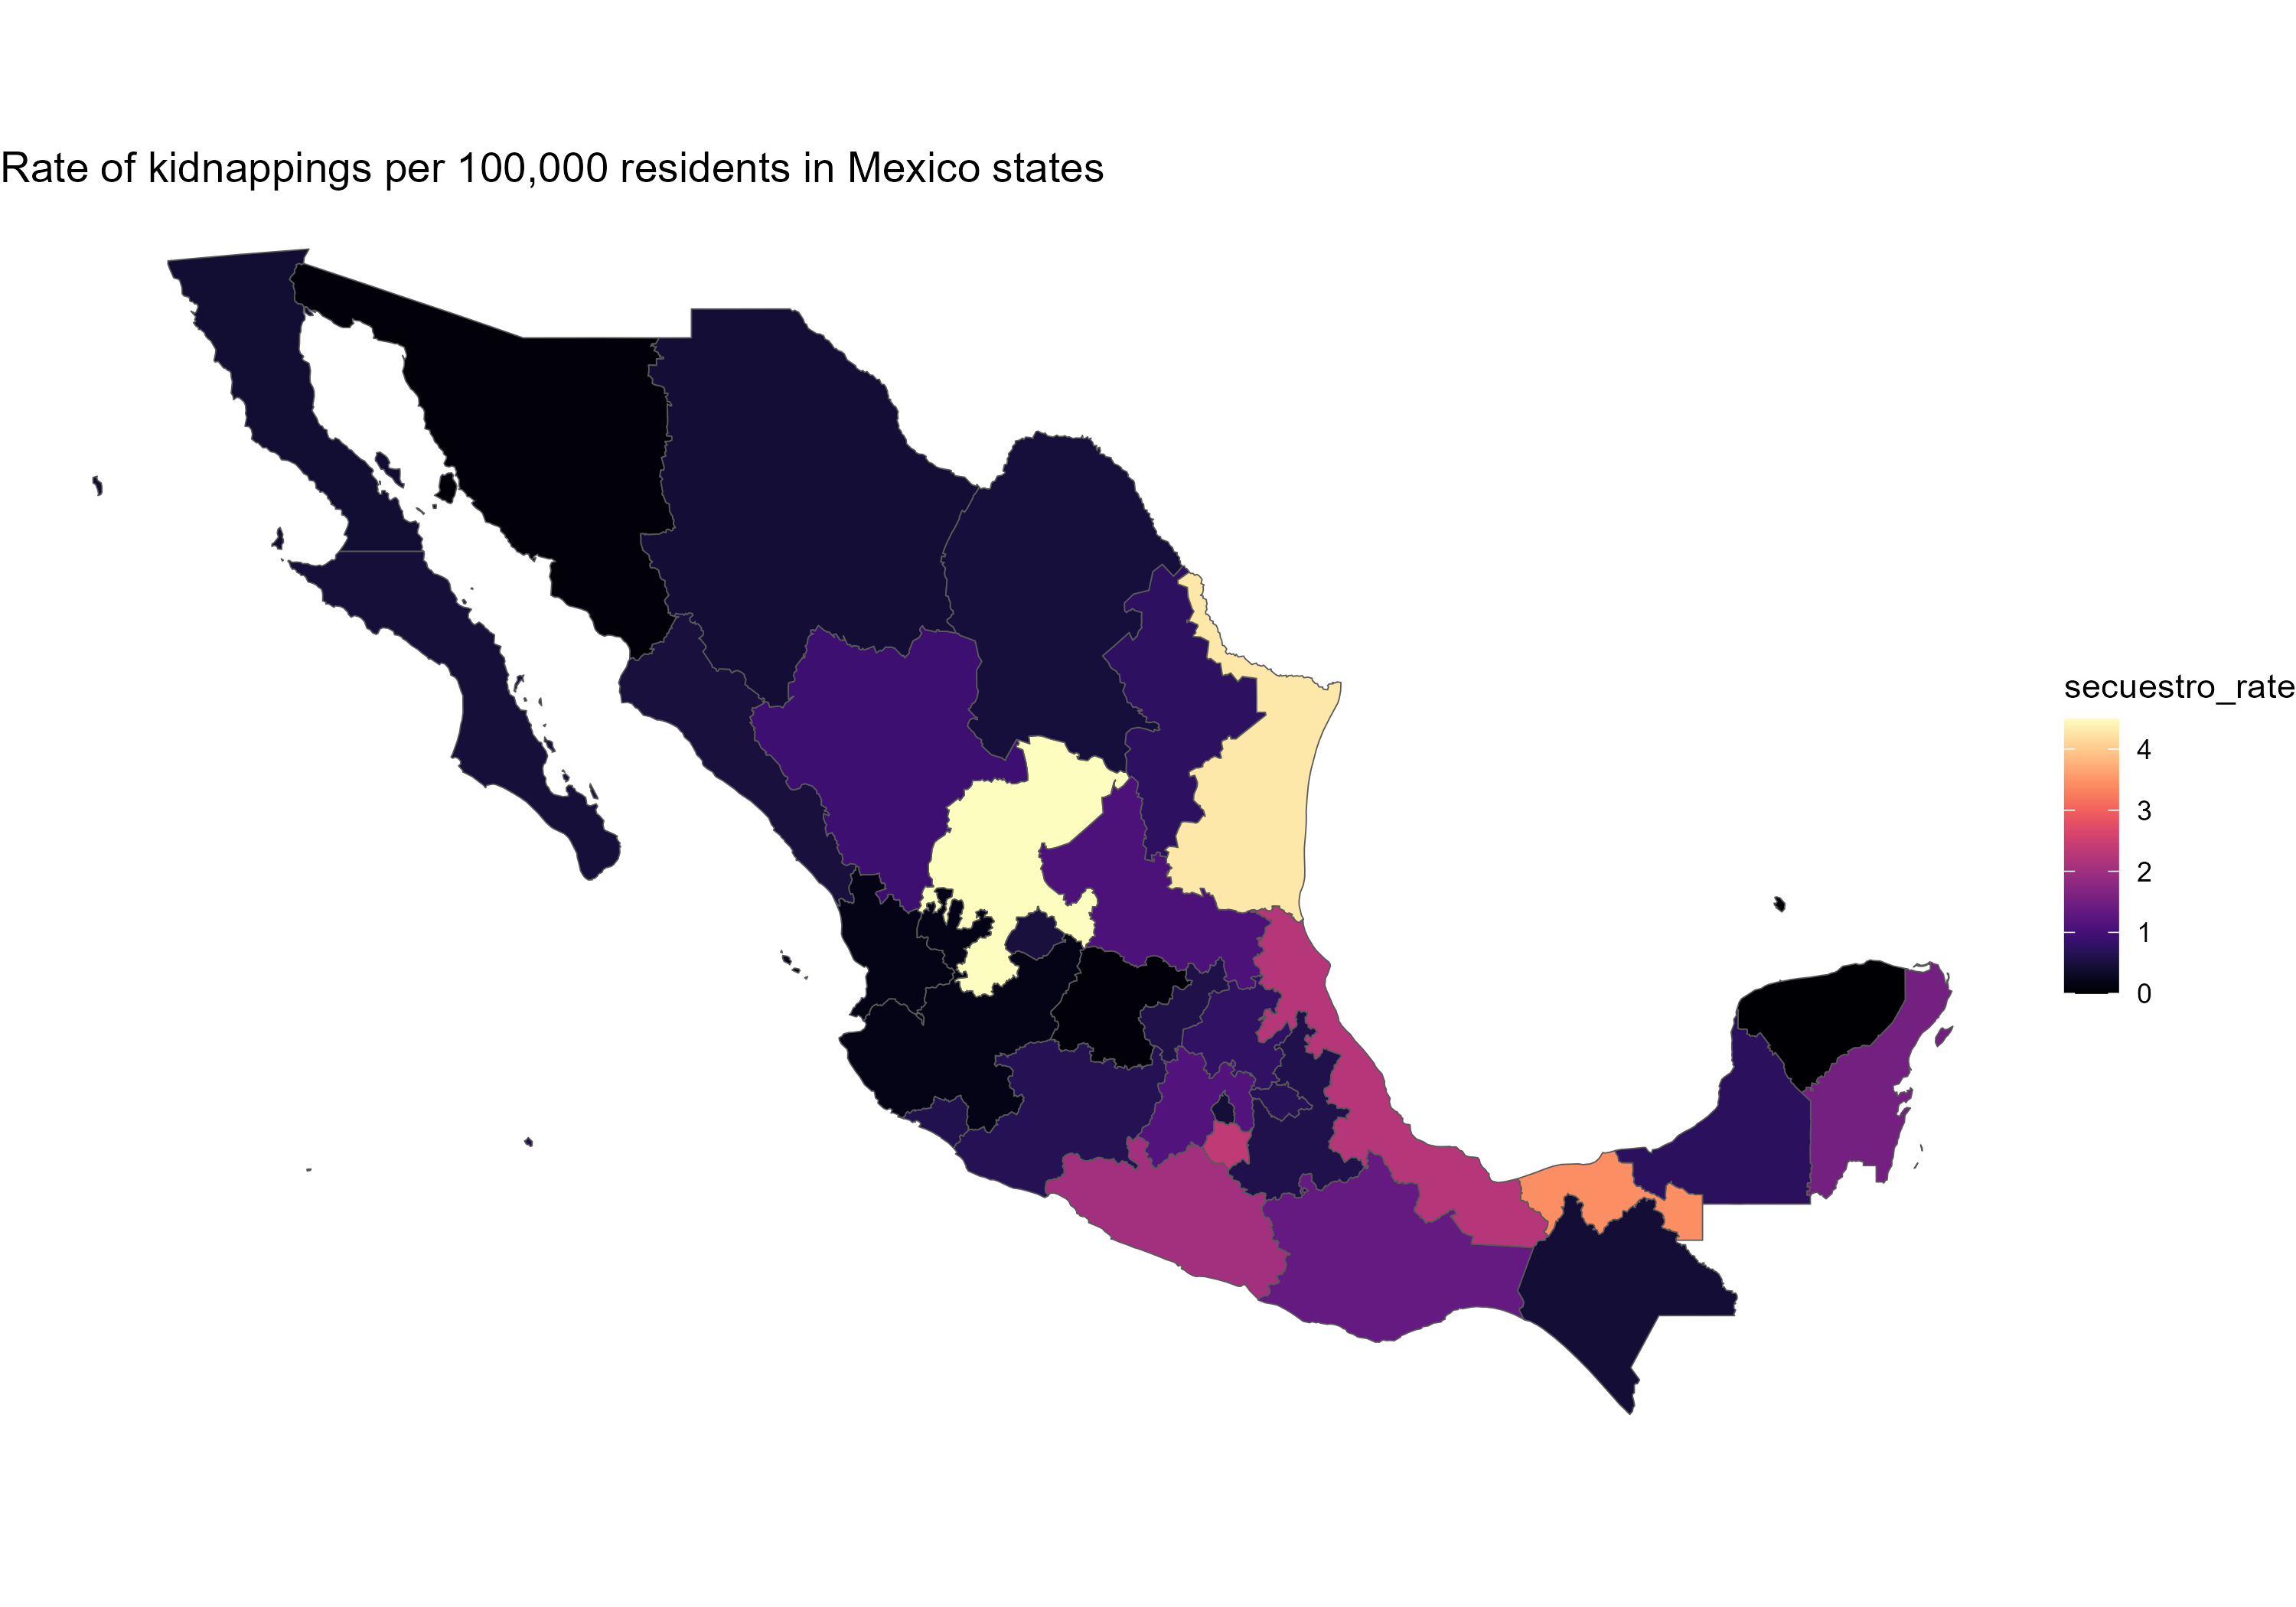
\includegraphics[width=41.67in]{exemplar-activities/Mexico_map}

XXXX

\textbf{References}

\end{document}
